\documentclass{beamer}
\usepackage{tikz}
\usepackage{array}
\usepackage{enumitem}
\usepackage{xcolor}
\usepackage{amsmath}
\usetikzlibrary{automata,positioning,arrows.meta,backgrounds}

% Define colors
\definecolor{myblue}{RGB}{0,0,255}
\definecolor{mypurple}{RGB}{128,0,128}
\definecolor{mygreen}{RGB}{0,128,0}
\definecolor{myorange}{RGB}{255,140,0}
\definecolor{lightblue}{RGB}{173,216,230}
\definecolor{peach}{RGB}{255,218,185}
\definecolor{lightpurple}{RGB}{230,230,250}

\usetheme{default}
\setbeamertemplate{navigation symbols}{}

\begin{document}

% First Slide - Branches and Performance
\begin{frame}
\frametitle{\textcolor{myblue}{Branches and Performance}}

\begin{itemize}
    \item[$\diamond$] \textbf{Misprediction Rate (MPR) vs. Misprediction Per Instruction (MPI)}
\end{itemize}

\vspace{0.3cm}

\begin{center}
\begin{tabular}{ccc}
$\text{MPR} = \dfrac{\text{\# mis-predicted jumps}}{\text{total \# jump}}$ & \hspace{1cm} & $\text{MPI} = \dfrac{\text{\# mis-predicted jumps}}{\text{total \# instructions}}$
\end{tabular}
\end{center}

\vspace{0.3cm}

\begin{itemize}
    \item[$\checkmark$] MPI correlates better with performance since it takes into account jumps frequency
\end{itemize}

\vspace{0.2cm}

\begin{itemize}
    \item[$\diamond$] \textbf{Assume}
    \begin{itemize}
        \item[$\checkmark$] MPI = 1\% (1 flush every 100 instructions on average)
        \item[$\checkmark$] IPC=2 \hspace{0.5cm} (2 instructions per cycle on average)
        \item[$\checkmark$] Flush penalty of 10 cycles
    \end{itemize}
\end{itemize}

\vspace{0.2cm}

\begin{itemize}
    \item[$\diamond$] \textbf{We get:}
    \begin{itemize}
        \item[$\checkmark$] MPI = 1\% $\Rightarrow$ 1 flush every 100 instructions on average
        \item[$\checkmark$] IPC=2 $\Rightarrow$ 1 flush every 50 cycles
        \item[$\checkmark$] 10 cycles flush penalty every 50 cycles
        \item[$\checkmark$] 20\% in performance
    \end{itemize}
\end{itemize}

\end{frame}

% Second Slide (previously first)
\begin{frame}
\frametitle{\textcolor{myblue}{Bimodal Predictor (cont.)}}

\vspace{-0.2cm}

\begin{center}
\textcolor{myblue}{\textbf{2-bit-sat counter array}}
\end{center}

\vspace{0.2cm}

\begin{center}
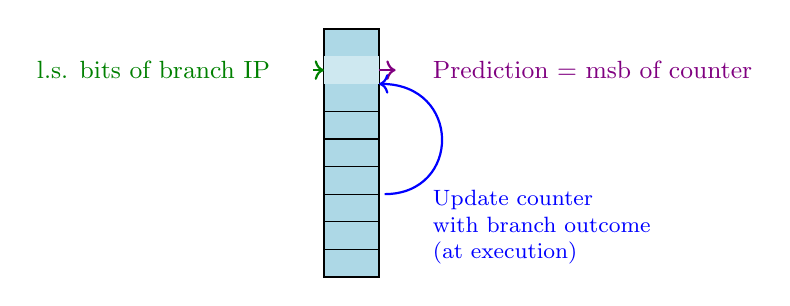
\begin{tikzpicture}[scale=0.7]
    % Draw the counter array
    \fill[lightblue] (0,0) rectangle (1,4.5);
    \draw[thick] (0,0) rectangle (1,4.5);
    
    % Draw array divisions
    \foreach \y in {0.5,1,1.5,2,2.5,3,3.5,4} {
        \draw (0,\y) -- (1,\y);
    }
    
    % Highlight the second cell from top (the one being accessed)
    \fill[lightblue!60] (0,3.5) rectangle (1,4);
    
    % Labels and arrows - pointing to second cell from top
    \node[mygreen,anchor=east,font=\small] at (-0.8,3.75) {l.s. bits of branch IP};
    \draw[->,thick,mygreen] (-0.2,3.75) -- (0,3.75);
    
    \node[mypurple,anchor=west,font=\small] at (1.8,3.75) {Prediction = msb of counter};
    \draw[->,thick,mypurple] (1,3.75) -- (1.3,3.75);
    
    % Curved arrow for update - starting low and curving up to second cell
    \draw[->,thick,myblue] (1.1,1.5) .. controls (2.5,1.5) and (2.5,3.5) .. (1,3.5);
    \node[myblue,align=left,anchor=west,font=\footnotesize] at (1.8,0.9) {Update counter\\with branch outcome\\(at execution)};
\end{tikzpicture}
\end{center}

\vspace{0.3cm}

\begin{itemize}
    \item[$\diamond$] \small\textbf{2-bit predictor avoids a double mistake in loops / glitches from the pattern}
\end{itemize}

\vspace{0.1cm}

{\footnotesize
\begin{tabular}{@{}ll@{}}
Branch Outcome & \texttt{0 0 0 0 0 1 0 0 0 0 0 1 0 0 0 0 0 1} \\
Prediction & \texttt{?~0 0 0 0 \textcolor{red}{0} 0 0 0 0 0 \textcolor{red}{0} 0 0 0 0 0 0} \\
\end{tabular}
}

\end{frame}


% Third Slide (previously second)
\begin{frame}
\frametitle{\Large\textcolor{myblue}{Bimodal (2-bit) Predictor}}

%\vspace{-0.3cm}

% Indent bullet points and allow more horizontal space
\setlist[itemize]{left=0.5em, rightmargin=0.5em}
\begin{itemize}
    \item[$\diamond$] \textbf{A 2-bit counter avoids the double mistake in glitches}
    \begin{itemize}
        \item[$\circ$] Need "more evidence" to change prediction
    \end{itemize}
\end{itemize}

\vspace{-0.2cm}

\begin{center}
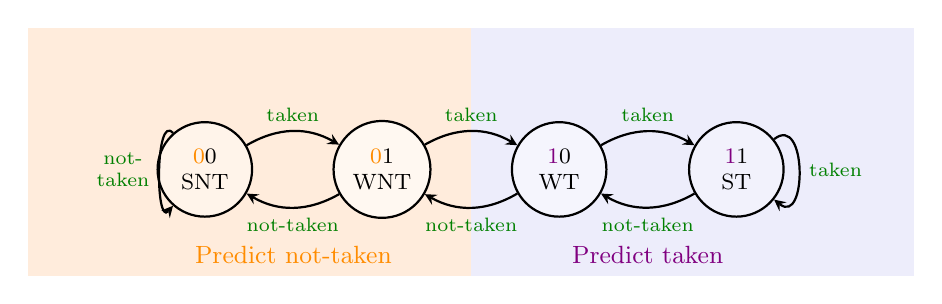
\begin{tikzpicture}[
    state/.style={circle,draw,thick,minimum size=1.2cm,font=\footnotesize,align=center},
    arrow/.style={->,>=stealth,thick},
    scale=0.9
]
    % Distinct background shades for prediction regions
    \begin{scope}[on background layer]
        \fill[peach!50] (-2.5,-1.5) rectangle (3.75,2); % Predict not-taken region
        \fill[lightpurple!70] (3.75,-1.5) rectangle (10,2); % Predict taken region, extended further right
    \end{scope}
    
    % States (LSB in black)
    \node[state,fill=peach!30] (SNT) at (0,0) {\textcolor{myorange}{0}\textcolor{black}{0}\\SNT};
    \node[state,fill=peach!20] (WNT) at (2.5,0) {\textcolor{myorange}{0}\textcolor{black}{1}\\WNT};
    \node[state,fill=lightpurple!40] (WT) at (5,0) {\textcolor{mypurple}{1}\textcolor{black}{0}\\WT};
    \node[state,fill=lightpurple!50] (ST) at (7.5,0) {\textcolor{mypurple}{1}\textcolor{black}{1}\\ST};
    
    % Self loop for SNT: from top left to bottom left, label on two lines
    \draw[arrow] (SNT) .. controls (-0.7,0.8) and (-0.7,-0.8) .. node[left,mygreen,font=\scriptsize,align=center] {not-\\taken} (SNT);
    % Self loop for ST: from top right to bottom right
    \draw[arrow] (ST) .. controls (8.5,0.8) and (8.5,-0.8) .. node[right,mygreen,font=\scriptsize,align=center] {taken} (ST);
    
    % Transitions between states
    \draw[arrow] (SNT) to[bend left=30] node[above,mygreen,font=\scriptsize] {taken} (WNT);
    \draw[arrow] (WNT) to[bend left=30] node[below,mygreen,font=\scriptsize] {not-taken} (SNT);
    
    \draw[arrow] (WNT) to[bend left=30] node[above,mygreen,font=\scriptsize] {taken} (WT);
    \draw[arrow] (WT) to[bend left=30] node[below,mygreen,font=\scriptsize] {not-taken} (WNT);
    
    \draw[arrow] (WT) to[bend left=30] node[above,mygreen,font=\scriptsize] {taken} (ST);
    \draw[arrow] (ST) to[bend left=30] node[below,mygreen,font=\scriptsize] {not-taken} (WT);
    
    % Prediction labels
    \node[myorange,font=\small] at (1.25,-1.2) {Predict not-taken};
    \node[mypurple,font=\small] at (6.25,-1.2) {Predict taken};
\end{tikzpicture}
\end{center}

\vspace{0.1cm}

\begin{itemize}
    \item[$\circ$] Initial state: weakly-taken (most branches are taken)
\end{itemize}

\begin{itemize}
    \item[$\diamond$] \textbf{Update (at execution)}
    \begin{itemize}
        \item[$\circ$] Branch was actually taken: increment counter (saturate at 11)
        \item[$\circ$] Branch was actually not-taken: decrement counter (saturate at 00)
    \end{itemize}
\end{itemize}

\begin{itemize}
    \item[$\diamond$] \textbf{Predict according to m.s.bit of counter (0=NT, 1=taken)}
    \item[$\diamond$] \textbf{Does not predict well branches with patterns like 010101...}
\end{itemize}

\end{frame}

\end{document}